%\chapter{Topology in quantum mechanics}
\label{sec:no_flat}
In mathematics, topology is concerned with the properties of a geometric object that are preserved under continuous deformations, such as stretching, twisting, crumpling, and bending; that is, without closing holes, opening holes, tearing, gluing, or passing through itself.\\
\begin{wrapfigure}{r}{.5\textwidth}
    \includegraphics[width=.6\textwidth]{Immagini/topo/topo1.pdf}
    \caption{The origin in represented with a black dot. On the left the different equivalence classes are shown in different colors}
    \label{fig:topo1}
\end{wrapfigure} 
Let's start with a simple but important example (figure \ref{fig:topo1}):
Let's consider the set of all the curves in the plane that do not pass thought the origin and that do not intersect themselves. We can divide this set in two main subsets:
\begin{itemize}
    \item The set of curves that circle around the origin (in orange)
    \item The set of curves that do not circle around the origin (in blue)
\end{itemize}
You cannot deform continuously a orange curve in to a blue one without crossing the origin, but you can deform continuously a curve to reach one of the same color, so we say that the two types of curves have different topologies, or alternatively that they form two different classes of equivalence.

As you can see from the image below, if we add noise, most of the time the curves will keep their topology. However, if the noise is strong enough, or the curve close enough to the origin, the curve sometimes changes its topology.
\begin{figure}[h]
    \includegraphics[width=\linewidth]{Immagini/topo/topo2.pdf}
    \caption{In this image the blue curve sometimes under noise keeps its topology, leaving its color unchanged, other times it gets pushed beyond the origin and switches color  (here shown in fuchsia)
    }
    \label{fig:topo2}
\end{figure}

\subsubsection*{Why is it important?}
For a physicist, things that are inherently topological in nature are important because they are resistant to noise. For example, in quantum computing the main bottleneck comes from environment noise. Because of this researchers are trying to explore the possibility of using topological effects to execute noise-resistant computations.




\section{Topology and Hamiltonians}
    In condensed matter physics we can ask whether the Hamiltonian of two quantum systems can be continuously transformed into each other. If that is the case, then we can say that two systems are \textit{topologically equivalent}.
    
    Clearly, every Hamiltonian could be continuously deformed into every other Hamiltonian with the same number of degrees of freedom. This changes drastically if we restrict ourselves to systems with an energy gap. This means that there is a finite energy cost to excite the system above its ground state. If an energy gap is present, then the Hamiltonian of the system has no eigenvalues in a finite interval around zero energy.


    \begin{figure}[h]
        \centering
        \includesvg{Immagini/topo/ham-path-1.svg}
        \caption{
        In this graph we show how the spectrum of the Hamiltonian changes as we move along a linear path between two randomly generated $10\times 10$ Hamiltonians $H(\alpha)=\alpha H_1+ (1-\alpha)H_0$, so $H(0)=H_0$ and $H(1)=H_1$
        In this case the two Hamiltonians are non-equivalent. Image taken from \cite{topocondmat}}
        \label{fig:ham-path-1}
    \end{figure}    
    
    We can now create the following topological classes of equivalence: we say that two gapped quantum systems are topologically equivalent if their Hamiltonians can be continuously deformed into each other without ever closing the energy gap.
    
    In order to know whether there is a any path which connects two Hamiltonians $H$ and $H'$ without closing the gap, we can count the number of filled energy levels. This is possible because the eigenvalues of gapped Hamiltonians can move freely as long as they don’t cross zero energy. Therefore continuous transformations exist exactly between Hamiltonians with the same number of energy levels below zero.
    
    Since the number of filled levels does not change under continuous transformations inside the set of gapped Hamiltonians we call it the \textit{topological invariant} $Q$. As you might expect, symmetries play an important role in determining topological equivalence classes, here we are going to explore some of them to 


\subsection*{Block diagonal symmetry}
If a Hamiltonian is symmetric under the unitary operator $U=\sigma_z\otimes \mathbb I$ it means that it can be written in block-diagonal form
\begin{equation}
    H=
    \begin{bmatrix}
    H_0 & \boldsymbol 0\\
    \boldsymbol 0 & H_1\\
    \end{bmatrix}
    \quad
    \rightarrow
    \quad U^\dag H U=H\,,
\end{equation}

where $H_0$ and $H_1$ are matrices with the same size, this means that the system as a whole behaves like two independent systems, each with its topological invariant $Q_i$.
Since the spectrum of the Hamiltonian $H$ is the union of the spectrum of the Hamiltonians $H_0$ and $H_1$, it means that the number of filled states of $H$ (which, by definition is $Q$) is the sum of the number of filled states of $H_1$ and $H_2$ ($Q_1$ and $Q_2$), so we have that 

\[
Q=Q_1+Q_2.
\]
However this symmetry, without anything extra does not yield interesting topologies, it only allows us to reduce the dimension of the problem.

\subsection*{Time reversal symmetry}
For systems with spin $1/2$ the time reversal operator has the form \cite{tong2017quantum2}

\begin{equation}
    \mathcal T=i\sigma_y\mathcal K\,,
\end{equation}
With $\sigma_y$ acting on the spin degree of freedom and where $\mathcal K$ is the complex conjugation operator. In that case $\mathcal T^2=-1$.
The Hamiltoninas with this kind of time-reversal symmetry obey the equation 
\begin{equation}
    H=\sigma_y H^* \sigma_y\,.
\end{equation}
Hamiltonian of this kind have every energy eigenvalues doubly degenerate (Kramer's degeneracy), so $Q$ can only have in the end even values. Intuitively this is because particles with spin up behave like particles with spin down, so they have the same energy.
% One way to explain this intuitively is that under time reversal the spin $\vect s$ changes sign
% \begin{equation}
%     \mathcal T^\dag \vect s\mathcal T=-\vect s
% \end{equation}
% If we 

\subsection*{Sublattice symmetry}
    Let’s now take a system where we can split all the degrees of freedom into two groups (say group A and group B) such that the Hamiltonian only has nonzero matrix elements between two groups, and not inside each group.
    
    This naturally arises in crystal systems with sublattice symmetry like graphene (we'll talk about graphene in detail further on). The Hamiltonian has the form
    
    \begin{equation}
        H=\begin{bmatrix}
        \vect 0 & H_{AB}\\
        H_{AB}^\dag & \vect 0
        \end{bmatrix}\,.
        \label{eq:sublattice-ham}
    \end{equation}
    If we define $\sigma_z$ such that it acts on the sublattice degree of freedom
    \begin{equation}
        \sigma_z
        \begin{bmatrix}
        \vect \psi_A\\
        \vect \psi_B
        \end{bmatrix}=
        \begin{bmatrix}
        \vect \psi_A\\
        -\vect \psi_B
        \end{bmatrix}\,,
    \end{equation}
    We have that
    \begin{equation}
        \sigma_z H \sigma_z=-H\,.
    \end{equation}
    This means that if $[\psi_A,\psi_B]^T$ is an eigenvector with energy $E$, then $[\psi_A,-\psi_B]^T$ is an eigenvector with energy $-E$

    \begin{figure}[h]
        \centering
        \includesvg[width=0.8\textwidth]{Immagini/topo/ham-path-2.svg}
        \caption{
        In this graph we show how the spectrum of the Hamiltonian changes as we move along a linear path between two randomly generated Hamiltonians in the form of equation \ref{eq:sublattice-ham} $H(\alpha)=\alpha H_1+ (1-\alpha)H_0$, so $H(0)=H_0$ and $H(1)=H_1$. As you can see the gap never closes. Image taken from \cite{topocondmat}}
        \label{fig:ham-path-2}
    \end{figure}  
    One way to show why the gap never closes is the following:
    We can take the Hamiltonian of equation \ref{eq:sublattice-ham} and decompose the two sublattice Hamiltonians with the \textit{singular value decomposition} 
    \begin{equation}
        H=U\Sigma V^\dag\,,
    \end{equation}
    where $U$ and $V$ are $n\times n$ unitary matrices and $\Sigma$ is a $n\times n$ diagonal matrix. If we want to find a path that goes from $H_0$ to $H_1$ in such a way that it never crosses the zero we just need to deform each one of the three matrices $U,\Sigma$ and $V$ in such a way that singular values do not appear in the path.
\subsection*{Particle-hole symmetry}
    Particle-hole symmetry shows up in superconducting systems, its Hamiltonian has the form of 
    \begin{equation}
        \mathcal H = \sum_{nm}H_{nm}c^\dag_nc_m+\frac 12
        \left(
             \Delta_{nm}c_n^\dag c_m^\dag+\Delta^*_{nm}c_n c_m,
        \right)\,,
        \label{eq:supeconduct1}
    \end{equation}
    where $c_n^\dag$ and $c_n$ are the creation and annihilation operators of the electrons in the state $n$. These operators follow the standard anticommutation rule
    \begin{equation}
        \{c_n,c_m\}=c_nc_m+c_mc_n=0
        \quad
        \{c_n^\dag,c_m\}=c_n^\dag c_m+c_mc_n^\dag=\delta_{nm}\,.
    \end{equation}
    We can group all the creation and annihilation operators in a vector \[C=[c_1,\dots,c_n,c_1^\dag,\dots,c_n^\dag]\,.\]
    We can now write $\mathcal H$ in a more compact way
    
    \begin{equation}
        \mathcal H=\frac 12 C^\dag H_{BdG}C\,.
    \end{equation}
    The matrix $H_{BdG}$ is knwon as the \texit{Bogoliuvov-de Gennes Hamiltonian}
    \begin{equation}
        H_{BdG}=
        \begin{bmatrix}
        H&\Delta\\
        -\Delta^*&-H^*
        \end{bmatrix}\,,
    \end{equation}
    Where the matrices $H$ and $\Delta$ are defined in equation \ref{eq:supeconduct1}. $H_{BdG}$ has the symmetry on exchange of electrons with holes, and there is an antiunitary operator for it $\mathcal P=\tau_x\mathcal K$ where the Pauli matrix $\tau_x$ acts on the particle and hole blocks and $\mathcal K$ is the complex conjugation operator. He have that
    \begin{equation}
        \mathcal P H_{BdG}\mathcal P^{-1}=-H_{BdG}\,.
    \end{equation}
    As you can see from figure \ref{fig:ham-path-3} the energy eigenvalues are symmetric around the zero energy. this is because if $[\vect \psi_1,\vect \psi_2]^T$ is an eigenvector with energy $E$, then $[\vect \psi_2^*,\vect \psi_1^*]^T$ is an eigenvector too, but with energy $-E$
    
    \begin{figure}[h]
        \centering
        \includesvg[width=0.7\textwidth]{Immagini/topo/ham-path-3.svg}
        \caption{
        In this graph we show how the spectrum of the Hamiltonian changes as we move along a linear path between two randomly generated Bogoljubov-de Gennes Hamiltonians in the form of equation \ref{eq:supeconduct1}. This time, however the gap closes from time to time.}
        \label{fig:ham-path-3}
    \end{figure}  

    The reason why this crossings come up is because the Bogoljubov-de Gennes Hamiltonian we had to double the degrees of freedom by introducing the holes. Hence a pair of $\pm E$ energy states does not correspond to two distinct quantum states, but to a single quantum state. This state is called a \textit{Bogoljubov quasiparticle} and it is a superposition of electron and hole
    \begin{equation}
        b^\dag=uc^\dag+vc\,.
    \end{equation}
    The levels sometime cross the zero because some times adding a Bogoljubov quasi particle requires energy, and sometimes it realises energy, when transitioning from one to the other you get a crossing.
    
    Clearly using the topological invariant $Q$ defined above would only give us trivial results, what we want is some kind of number that changes when there is a level crossing. The Eigenvalues of $G_{BdG}$ always come in pairs $\pm E$, so it is equal to 
    
    \[
        \det\left(H_{BdG}\right)=\prod_n -E_n^2\,.
    \]
    If we take the square root of the determinant in such a way that its sign is uniquely determined, also called the \textit{Pfaffian}\footnote{Actually it is a bit more complicated than taking the square root. The Pfaffian is a property of asymmetric matrices, and $H_{BdG}$ it is not, however though a change of basis it can be cast into one}, we can define the following topological invariant 
    \begin{equation}
        Q_{BdG}=\sign\left[\textrm{Pf}(iH_{BdG})\right]\,.
    \end{equation}
    The results of computing the Pfaffian can be seen in figure \ref{fig:ham-path-3}
    

\section{Edge states and the bulk-boundary correspondence}

    A fundamental consequence of the topological classification of gapped states is the emergence of gapless conducting states at interfaces where the topological invariant changes. This edge states are present at the interface between integer Hall state and vacuum  \cite{halperin1982quantized}. These states can be understood in terms of the skipping motion electrons execute as their cyclotron motion bounce off the edge Arguably the most important property of edge states is their \textit{chirality} in the sense that they only propagate in one direction along the edge. These states are insensitive to disorder because there are no states available for backscattering.
    \begin{figure}[h]
        \centering
        \includegraphics[width=\textwidth]{Immagini/topo/edge_sates.pdf}
        \caption{
        In the figure on the left (a) the edge mode is represented as an electron in a skipping motion. On the right (b) is shown the electronic structure of a topological material and the line that unites the conduction band with the valence band represents the edge state. Image taken from \cite{hasan2010colloquium}}
        \label{fig:edge}
    \end{figure}\\
    The existence of these one way states are linked to the existence of the topological numbers. If to go from one topological number to the other you need to close the gap, then if we start form inside one material, and we end up to the other material, somewhere along the way the gap has to close and the only reasonable place to do so is the boundary \cite{jackiw1976vacuum}. Keep in mind that one of the two materials can be the vacuum itself 
    

        
\section{Spectral Flow}
    
        
        Another example of topology in quantum mechanics is the concept of \textit{spectral flow}. To start off we are going to talk about a very specific case of a quantum particle in a ring around a infinitely long solenoid.\\
        The Hamiltonian of a particle with charge $-e$ moving through a magnetic field $\mathbf B= \nabla \times \mathbf A$ is
        \begin{equation} \label{EMHamiltonian}
                H=\frac 1{2m}(\mathbf p + e\mathbf A)^2 \,.
        \end{equation}
        \begin{wrapfigure}{r}{.4\textwidth}
            \includegraphics[width=.4\textwidth]{Immagini/topo/solenoid.pdf}
            \caption{Particle in a ring threaded by a solenoid}
        \end{wrapfigure} 
        Since 
        \[
            \mathbf p=p_\theta \hat\theta=-\frac{i\hbar\mathbf {\hat \theta}}{R}\frac\partial {\partial \theta}\,,
        \]
        \[
            \oint \mathbf A\cdot d\mathbf r=\int \mathbf B\cdot d\mathbf s = \Phi\,,
        \]   
        it means that
        \begin{equation} \label{vector_potential}
            \mathbf A=\frac \Phi{2\pi R} \mathbf {\hat \theta}\,.
        \end{equation}
        Putting it back into the Hamiltonian
        \begin{equation} \label{EMHamiltonian2}
            H=\frac 1{2m}\bigg(-\frac{i\hbar}{R}\frac\partial {\partial \theta} + \frac{e\Phi}{2\pi R}\bigg)^2 \,.
        \end{equation}
        The eigenstates of this Hamiltonian are 
        \[
            \psi_n(\theta)=\frac {e^{in\theta}} {\sqrt{2\pi R}}; \quad n\in \mathbb Z\,.
        \]
        Interestingly the Energies of the eigenstates are influenced by the vector potential
        \begin{equation} \label{spectral_flow}
                E_n=\frac 1{2mR^2}\bigg(\hbar n+ \frac{e\Phi}{2\pi}\bigg)^2=\tilde E\bigg(n+\frac{\Phi}{\Phi_0}\bigg)^2\,,
        \end{equation}
        where
        \[
        \tilde E=\frac{\hbar^2}{2mR^2} \quad \textrm{and} \quad \Phi_0=\frac{2\pi \hbar}e\,.
        \]
        Suppose now that we start with the turned solenoid off, and place the particle in the $n=0$ ground
        state. If we increase the flux then, by the time we have reached $\Phi=\Phi_0$ , the $n=0$ state
        has transformed into the state that we previously labelled $n = 1$. Similarly, each state
        $n$ is shifted to the next state, $n + 1$ \footnote{It is tempting to invoke the adiabatic theorem
        here but, because of level crossing at $\Phi=\Phi_0/2$ it is not valid}.\\
        \begin{minipage}{\textwidth}
         \includegraphics[width=1\linewidth]{Immagini/topo/flow.pdf}
        \end{minipage}
        This is an example of a phenomenon is called spectral flow: under a change of parameter
        the spectrum of the Hamiltonian changes, or “flows”. As we change increase the flux
        by one unit  $\Phi_0$ the spectrum returns to itself, but individual states have morphed into
        each other. \cite{tong2016lectures}
        \begin{figure}[h]
            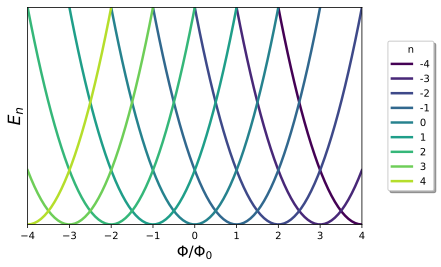
\includegraphics[width=\linewidth]{Immagini/topo/spectral_flow.pdf}
            \caption{Here plotted the energies $E_n$ (eq. \ref{spectral_flow} ), notice how the states \textit{"flow"} as we change $\Phi$. Image adapted from \cite{tong2016lectures}}
            \label{fig:spectral-flow}
        \end{figure}
    \subsection*{Parallelism with Bloch's Theorem}
    
        You might have noticed that figure \ref{fig:spectral-flow} is suspiciously similar to a crystal band structure in the limit on which the periodic potential $V\to 0$ with periodicity $2\pi$, let us see if this analogy holds \textit{the test of math}. Let's start by taking the single-particle free propagating Hamiltonian 
        \[
            H=\frac 1{2m}p_\theta^2\,.
        \]
        The eigenstates this time have to respect the condition that 
        \begin{equation}
        u_{n,q}(\theta)=e^{i2\pi q}u_{n,q}(\theta+2\pi)\,.
        \end{equation}
        This also means that if we substitute $q\to q+1$ the spectrum doesn't change.\footnote{This come from the Bloch's theorem that states that the eigenstates of the Hamiltonian of a periodic potential with periodicity $a$ mush obey that $u_{n,q}(x)=e^{iaq}u_{n,q}(x+a)$. In our case the periodicity $a=2\pi$ and the variable of the function is $\theta$ instead of $x$}\\
        % \begin{addmargin}[2em]{2em}
        %     \subsubsection*{Brief proof}
        %     A brief proof of this is the following:\\
        %     The problem of the eigenvalues can be written like so 
        %     \[
        %         He^{iq\theta}u_{n,q}(\theta)=E_n(q)e^{iq\theta}u_{n,q}(\theta)
        %     \]
        %     if we now send $q\to q+1$ the equation above becomes
        %     \[
        %         He^{iq\theta}e^{i\theta}u_{n,q+1}(\theta)=E_n(q+1)e^{iq\theta}e^{i\theta}u_{n,q+1}(\theta)
        %     \]
        %     The terms $u'_{n,q}(\theta)\equiv e^{i\theta}u_{n,q+1}(\theta)$ are also periodic $u'_{n,q}(\theta)=u'_{n,q}(\theta+2\pi)$. If we put it back into the equation above we get
        %     \[
        %         He^{iq\theta}u'_{n,q}(\theta)=E_n(q+1)e^{iq\theta}u'_{n,q}(\theta)
        %     \]
        %     That is completely equivalent to the equation at the start of this footnote, this means that the eigenvalues are periodic with periodicity 1\\
        % \end{addmargin}
        We now make the following unitary transformation to obtain a $q$-depentant Hamiltonian.
        \[
            H(q)=e^{-iq\theta}He^{iq\theta}=\frac 1{2m}\bigg (p_\theta + \frac {\hbar q}R \bigg)^2\,.
        \]
        We can easly map this hamiltonian to the one in equation \ref{EMHamiltonian2} just by difining $\Phi$ such that $\hbar q= \frac {e\Phi}{2\pi}$. 
        \begin{equation} \label{blochA}
            H(\Phi)=\frac 1{2m}\bigg(p_\theta + \frac{e\Phi}{2\pi R}\bigg)^2\,.
        \end{equation}
        Since before we said that the system doesn't change if we substitute $q\to q+1$, it means that now the system remains unchanged if we send $\Phi \to \Phi+\Phi_0$. This is exactly the result obtained in the previous page.
    
    
        And the tranformed eigenstates $\psi_{n,q}=e^{-iq\theta}u_{n,q}$ is just the cell-periodic part of the Bloch function. It satified the stricter periodic boundary condition
        \begin{equation} \label{blochboundraty}
            \psi_{n,q}(\theta)=\psi_{n,q}(\theta +2\pi)\,.
        \end{equation}
        As you can see equations \ref{blochA}  and \ref{blochboundraty} create a system that is mathematically equivalent to the particle moving in a ring around a flux tube \cite{WeinbergBloch}.






    \subsection*{Conditions to have spectral flow}
        Up until now we looked spectral flow the case where the particle is freely propagating, let's see what happens when we add a periodic potential $V(\theta)=V(\theta+2\pi)$
        \[
            H=\frac 1{2m}p_\theta^2 + V(\theta)\,.
        \]
        Now the spectrum is still periodic, however the energy bands do not necessarily cross, this means that  when abiabatically changing $q$, (or equivalently $\Phi$) the states won't flow, instead they will return to their original state.
        \begin{figure}[h]
            \includegraphics[width=\linewidth]{Immagini/topo/grosso-flow.png}
            \caption{Pictorial representation of what happens when changing $q$. Image taken from \cite{grosso2013solid}}
        \end{figure}\\
        Conversely if there are $n$ degeneracies, on every cycle more the $i$-th state will flow to the $i+n$-th state.\newpage


    
    \subsection*{Spectral flow in a more general context}
    
        The spectral flow is applicable in much more complex geometries than the one we have seen so far.\\
        Suppose that now the particle can moove in a 3D potential $V(\mathbf r)$, the Hamiltonian is
        \[
            H(\mathbf A)=\frac 1{2m}(\mathbf p + e\mathbf A)^2 + V(\mathbf r) \,,
        \]
        since the solenoid is still the same, the formula for $\mathbf A$ remains unchanged (eq. \ref{vector_potential} )
        \[
            H(\Phi)=\frac 1{2m}\bigg(\mathbf p + \frac{e\Phi}{2\pi R}\hat \theta\bigg)^2 + V(\mathbf r)\,,
        \]
        and since it's expressed in cylindrical coordinates it's better to express also $\mathbf p$ in cylindrical coordinates.
        \[
         \mathbf p =-i\hbar \mathbf \nabla=-i\hbar\bigg( 
             \mathbf{\hat r}\frac{\partial}{\partial r}+ \frac{\mathbf {\hat \theta}}{r}\frac{\partial}{\partial \theta} + \mathbf{\hat z}\frac{\partial}{\partial z}  \bigg) \equiv
             \mathbf{\hat r} p_r+ \mathbf {\hat \theta} p_\theta + \mathbf{\hat z} p_z\,.
        \]
        Of course if we send $\theta \to \theta + 2\pi$ the system should be unchanged.
        \[
            \psi(r,\theta,z)=\psi(r,\theta+2\pi,z)\,.
        \]
        Following the inverse reasoning done in the previous subsection we make the following unitary transformation
        \[
            H=e^{i\theta\Phi/\Phi_0}H(\Phi)e^{-i\theta\Phi/\Phi_0}=\frac  {\mathbf p^2} {2m} + V(\mathbf r)\,.
        \]
        This means that the eigenvalue problem is now written like so
        \[
            He^{i\theta\Phi/\Phi_0}\psi(r,\theta,z)=E(\Phi)e^{i\theta\Phi/\Phi_0}\psi(r,\theta,z)\,.
        \]
        If we send $\Phi \to \Phi+\Phi_0$ we get an equivalent equation
        \[
            He^{i\theta\Phi/\Phi_0}\psi(r,\theta,z)=E(\Phi+\Phi_0)e^{i\theta\Phi/\Phi_0}\psi(r,\theta,z)\,.
        \]
        This means that the energy spectrum is unchanged if we send $\Phi \to \Phi+\Phi_0$. This is true regardless of the shape or geometry of $V(\mathbf r)$.
        
    
    \subsection*{The quantum Hall effect}

    
    
        We'll now see the effects of the spectral flow on physical properties of materials. Suppose we have a system like the one of the figure on the side. Now we slowly increase $\Phi$ from 0 to $\Phi_0$ in a total time $T$. This introduces a electromagnetic force around the ring $\mathcal{E}=-\partial_t\Phi=-\Phi_0/T$.
        \begin{wrapfigure}{r}{.4\textwidth}
            \includegraphics[width=.4\textwidth]{Immagini/topo/disk-solenoid.pdf}
        \end{wrapfigure} 
        Due to spectral flow $n$ electrons are transferred form the inner circle to the outer circle in this time $T$. This would result in a radial current $I_r=-ne/T$. This means that the resistance is 
        \begin{equation} 
            \label{hall_resistivity}
                R_{xy}=\frac{\mathcal {E}}{I_r}=\frac{2\pi\hbar}{e^2}\frac 1n\,.
        \end{equation}
        In the case there is no spectral flow, it is equivalent as saying $n=0$, so this treatment works is still valid.\\
        To be able to calculate $n$ we need to calculate how is the spectrum of the system as we change $\Phi$. This means that $n$ depends on the system, but equation \ref{hall_resistivity} is independent of the system.\\
        This effect to be observed the system has to be in a definite quantum state, so in real life scenario the material has to be cooled to low enough temperatures.